\documentclass{article}
\usepackage{amsmath}
\usepackage[margin=0.5in]{geometry}
\usepackage{breakcites}
\usepackage{natbib}
\usepackage{mathtools}
\usepackage{mathrsfs}
\usepackage{graphicx}
\usepackage{caption}
\usepackage[bottom]{footmisc}
\usepackage[export]{adjustbox}
\usepackage{todonotes}
\usepackage{footnote}
\usepackage{threeparttable}

\usepackage{newfloat}
\DeclareFloatingEnvironment[placement={!ht},name=List]{ordlist}

\usepackage{xr}
\externaldocument[S-]{supplement}

\DeclarePairedDelimiter\ceil{\lceil}{\rceil}
\DeclarePairedDelimiter\floor{\lfloor}{\rfloor}
\DeclareMathAlphabet\mathbfcal{OMS}{cmsy}{b}{n}
\DeclareMathOperator*{\argmin}{arg\,min}

\begin{document}


\newcommand{\monosaccharide}[1]{{\bf #1}}
\newcommand{\nglycan}[0]{\textit{N}-glycan }
\newcommand{\nglycans}[0]{\textit{N}-glycans }

\newcommand{\msn}[0]{$MS^n$}
\newcommand{\ms}[1]{$MS^#1$}

% Sample Name Shortcuts
\newcommand{\agp}[0]{\textit{20150930-06-AGP} }
\newcommand{\phil}[0]{\textit{20141031-07-Phil-82} }
\newcommand{\philbs}[0]{\textit{20141101-04-Phil-BS} }
\newcommand{\igg}[0]{\textit{20151002-02-IGG} }
\newcommand{\dpphil}[0]{\textit{20141128-11-Phil-82} }
\newcommand{\dpagp}[0]{\textit{AGP-DR-Perm-glycans-1} }
\newcommand{\rpagp}[0]{\textit{AGP-permethylated-2ul-inj-55-SLens} }
\newcommand{\rphumanserum}[0]{\textit{Perm-BS-070111-04-Human-Serum} }


\title{Application of Network Smoothing to Glycan LC-MS Profiling}
\author{Joshua Klein}
\begin{abstract}
    \textbf{Motivation:} Glycosylation is one of the most heterogenous
    and complex post-translational modifications, but.\\
    \textbf{Results:} These are the resutls for this article.\\
\end{abstract}

\maketitle

\section{Introduction}
Glycosylation is one of the most pervasive forms of post-translational
modification.


\section{Methods}

\subsection{Glycan Hypothesis Generation}
    In eukaryotes, \nglycans start with a common, conserved core of \textbf{HexNAc2 Hex3},
    building up to \textbf{HexNAc2 Hex9} (\cite{Stanley2009}). This structure is refined by
    sequentially removing monosaccharides and replacing them with more complex structures
    through a series of glycosylase and glycosyltransferase reactions, the enumeration of,
    which as shown in \cite{Akune2016}, yields over a million of possible \nglycan topologies.
    These topologies define the geometry of the glycan, affecting the glycan's binding affinities
    and how the glycan may influence protein folding and accessibility, the glycan's functional
    aspects. The medium through which we observed glycans did not capture the full tree or
    graph structure of an \nglycan, so we reduced the topology to a count of each type of residue.

    Starting with the core motif, we generated all combinations of monosaccharides ranging
    between the limits in Table~\ref{tab:glycan_composition_rules} to build a glycan composition
    database, which produced 1240 distinct compositions. We created a copy of this database for
    native, reduced and permethylated, and deuteroreduced and permethylated for each experimental
    protocol we analyzed in this study. We chose to use a combinatorial database for simplicity.
    The later algorithms can be used with an arbitrary glycan composition list. This places the
    burden of finding or creating such a list on the user. The glycan database is stored in a
    SQLite3 (v3.15.2) database file (\cite{Hipp2016}).

    \begin{table}
        \small
        \centering
        \caption{Glycan Composition Rule Table}\label{tab:glycan_composition_rules}
        \begin{threeparttable}
        \begin{tabular}{c | c | c | c}
            \toprule
            Monosaccharide & Lower Limit & Upper Limit & Constraints\\
            \midrule
            \monosaccharide{HexNAc} & 2 & 9 &\\
            \monosaccharide{Hex} & 3 & 10 & \\
            \monosaccharide{Fuc} & 0 & 4 & $\monosaccharide{HexNAc} > \monosaccharide{Fuc}$\\
            \monosaccharide{NeuAc} & 0 & 5 & $(\monosaccharide{HexNAc} - 1) > \monosaccharide{NeuAc}$\\
        \end{tabular}
        \end{threeparttable}
    \end{table}


\subsection{LC-MS Data Preprocessing}
    We analyzed samples from several sources, including both QTOF and Orbitrap
    instruments as shown in Table \ref{tab:sample_overview}. For details on sample preparation
    and data acquisition, please see the source citations. We converted all
    datasets to mzML format (\cite{Martens2011}) using Proteowizard
    (\cite{Kessner2008}) without any data transforming filters. We applied a background reduction
    method based upon (\cite{Kaur2006}), using a window length of 2 m/z. Next, we picked peaks using
    a simple Gaussian model and iteratively charge state deconvoluted and deisotoped using an
    averagine (\cite{Senko1995}) formula appropriate to the molecule under study. For native
    glycans, the formula was \textbf{H 1.690 C 1.0 O 0.738 N 0.071}, for permethylated glycans,
    the formula was \textbf{H 1.819 C 1.0 O 0.431 N 0.042}. We used an iterative approach which combines
    aspects of the dependence graph method (\cite{Liu2010}) and with subtraction. All samples
    were processed using a minimum isotopic fit score of 20 with an isotopic strictness penalty
    of 2.

    \begin{table}
        \caption{Samples Used}\label{tab:sample_overview}
        \small
        \centering
        \begin{threeparttable}
        \begin{tabular}{p{4.1cm} | c | p{3cm} | p{3cm} | c}
            \toprule
            Sample Name & Instrument & Derivatization & Adduction & Source\\
            \midrule
            20150930-06-AGP & QTOF & Native & Formate (1) & \cite{Khatri2016a}\\
            20141031-07-Phil-82 & QTOF & Native & Formate (3) & \cite{Khatri2016a}\\
            20141103-02-Phil-BS & QTOF & Native & Formate (3) & \cite{Khatri2016a}\\
            20151002-02-IGG & QTOF & Native & Formate (2) & \cite{Khatri2016b}\\
            20141128-11-Phil-82\tnote{1} & QTOF &
                Deutero-reduced and Permethylated & Ammonium (3) & \cite{Khatri2016a}\\
            AGP-DR-Perm-glycans-1\tnote{1} & Orbitrap &
                Deutero-reduced and Permethylated & Ammonium (3) & \cite{Khatri2016a}\\
            AGP-permethylated-2ul-inj-55-SLens\tnote{1} & Orbitrap &
                Reduced and Permethylated & Ammonium (3) & \cite{Khatri2016a}\\
            Perm-BS-070111-04-Serum\tnote{1} & Orbitrap &
                Reduced and Permethylated & Ammonium (3) & \cite{Yu2013,Hu2012}\\
        \end{tabular}
        \begin{tablenotes}
            \item[1] Included $MS^n$ Scans
        \end{tablenotes}
        \end{threeparttable}
    \end{table}


\subsection{Chromatogram Aggregation}
    We clustered peaks whose neutral masses were within 15 parts-per-million error
    (PPM) of each other. When there were multiple candidate clusters for a single peak,
    we used the cluster with the lowest mass error. Next, we sorted each cluster by time,
    creating a list of aggregated chromatograms. To account for small mass differences,
    we found all chromatograms which are within 10 PPM of each other and which overlap
    in time and merge them.

\subsection{Glycan Composition Matching}
    For each chromatogram, we searched the glycan database for compositions
    whose masses were within $\delta_{mass} = 10$ PPM for QTOF data, $5$ PPM
    for FTMS data. We merged all features matching the same composition. Then, for
    each adduct combination, we searched the glycan database for compositions
    whose neutral mass were within $\delta_{mass}$ of the observed neutral mass - adduct
    combination mass, followed by another round of merging chromatograms with the same
    assigned composition. We reduced the data by splitting each feature where the time
    between sequential observation was greater than $\delta_{rt} = 0.25$ minutes and
    removed features with fewer than $k = 5$ data points.%
    % The MSn filter makes comparison with MultiGlycan-ESI difficult, so this doesn't
    % make sense to include here.
    % 
    % For cases where $MS^n$ scans were
    % present, these scans were mapped onto their precursor $MS^1$ features, and evaluated for
    % glycan-like product ions, retaining only those which satisfied the signature ion
    % criterion described in section S\ref{S-sec:signature_ion_criterion}.
    We term the remaining assigned and unassigned chromatograms \textit{candidate features}.


\subsection{Feature Evaluation}
        For each candidate feature, we computed several metrics to estimate
    how distinguishable the observed signal was from random noise. The
    features are mentioned in List~\ref{list:scoring_features}, but for more
    information see Section~S\ref{S-sec:feature_evaluation}.
    \begin{ordlist}
    \begin{enumerate}
        \itemsep0em
        \caption{Chromatographic Feature Metrics\label{list:scoring_features}}
        \item Goodness-of-fit of chromatographic peak shape to a model function
              (\cite{Yu2010,Kronewitter2014}).
        \item Goodness-of-fit of isotopic pattern to glycan composition weighted
              by peak abundance (\cite{Maxwell2012}).
        \item Observed charge states with respect to glycan composition and mass.
        \item Time gap between $MS^1$ observations detecting measuring missing peaks
              and interference.
        \item Adduction states with respect to glycan composition and mass.
    \end{enumerate}
    \end{ordlist}

        These metrics are bounded in $[0, 1)$. Any observation for which any metric
    was observed below $0.15$ was discarded as having insufficient evidence for
    consideration. The \textit{observed score} $s$ for each candidate feature is
    the sum of the logit-transformation of these metrics. This produces a single
    value bounded in $[0, \infty)$, whose distribution we assume is asymptotically
    normal. $s < 8$ reflects a low confidence match, with confidence increasing
    as $s$ does. As these metrics are tied to reliable detection of the the glycan
    by the mass spectrometer, they are dependent upon glycan abundance and sample
    quality and the resolution of the mass spectrometer used.


\subsection{Glycan Composition Network Smoothing}
        Evidence for individual glycan compostions can often be enough to claim
    that composition had been detected. Lower abundance may score poorly in one
    or more features, leading to the glycan composition being discarded. Other
    methods have demonstrated it is advantageous to use relationships between
    glycans based on biosynthetic or structural rules to adjust the score of a
    single glycan assignment (\cite{Goldberg2009, Kronewitter2014}). This idea
    has been explored more generically under the name "Manifold Regularization"
    (\cite{Belkin2006}) and specifically "Laplacian Regularization" when the
    Laplacian matrix of a graph is used to influence the parameter scaling. We
    apply this idea to weighted networks of related glycans with arbitrarily
    defined and overlapping sub-populations.

        \subsubsection{Glycan Composition Graph}
        For each database of theoretical glycan compositions we create, we
        define each composition to be a coordinate vector in a $\mathcal{Z}^{+c}$
        space where $c$ is the number of components in any glycan composition,
        and represented by a node in an undirected glycan composition
        graph $\mathcal{G}$. Under this interpretation, we can compute the
        $L_1$-distance between two glycan compositions, \reviewchange{representing the biosynthetic
        distance between the two compositions, an analog for the number of enzymatic
        steps needed to go from one glycan to the other}. For any two glycan
        compositions $g_u, g_v$, if $L_1(g_u, g_v) = 1$ we add an edge
        connecting $g_u$ and $g_v$ to $\mathcal{G}$ with weight $w = 1$.


        \subsubsection{Neighborhood Definition}
        Our definition of distance connects glycan compositions which differ
        by a single monosaccharide, but we can assert how larger collections of
        glycan compositions are related. To this end, we extend the definition of
        neighborhoods for \nglycans using intervals over monosaccharide counts
        shown in Table~\ref{tab:neighborhood_definitions}. These neighborhoods are
        arranged to span particular epitopes or biosynthetically related
        subtypes of \nglycans, such as sialylation state or branching
        pattern. \reviewchange{Neighborhoods overlap sets of glycan compositions which are also
        biosynthetically related. Each neighborhood spans the eponymous class of
        glycan compositions, as well as the preceding class and proceeding class.
        For example, For example, the Tri-Antennary neighborhood spans Bi-Antennary
        Tetra-Antennary compositions. This helps to channel the estimation of}
        $\mathbf{\tau}$ \reviewchange{among related groups.
        The Hybrid, Bi-Antennary and Asialo-Bi-Antennary neighborhoods introduce
        complications because they are biosynthetically close to each other. For the
        simplicity, we chose to include all of Hybrid in Asialo-Bi-Antennary
        and permit up to one NeuAc in it.}

        \begin{table}[tb]
            \scriptsize
            \begin{tabular}{l |S|S| S|S| S|S| S}
                \toprule
                \multirow{3}{*}{Name} & \multicolumn{2}{c|}{HexNAC} & \multicolumn{2}{c|}{Hex} & \multicolumn{2}{c|}{NeuAc} & \reviewchange{Size} \\
                                      &  {Min}        &    {Max}   &     {Min}   &    {Max}  &     {Min}     &    {Max}  &      \\
                \midrule
                High Mannose          &     2         &     2      &       3     &     10    &       0       &      0    &  16 \\
                Hybrid                &     2         &     4      &       2     &     6     &       0       &      2    &  80 \\
                Bi-Antennary          &     3         &     5      &       3     &     6     &       1       &      3    &  104\\
                Asialo-Bi-Antennary   &     3         &     5      &       3     &     6     &       0       &      1    &  96 \\
                Tri-Antennary         &     4         &     6      &       4     &     7     &       1       &      4    &  172\\
                Asialo-Tri-Antennary  &     4         &     6      &       4     &     7     &       0       &      0    &  56 \\
                Tetra-Antennary       &     5         &     7      &       5     &     8     &       1       &      5    &  240\\
                Asialo-Tetra-Antennary&     5         &     7      &       5     &     8     &       0       &      0    &  60\\
                Penta-Antennary       &     6         &     8      &       6     &     9     &       1       &      5    &  280\\
                Asialo-Penta-Antennary&     6         &     8      &       6     &     9     &       0       &      0    &  60\\
                Hexa-Antennary        &     7         &     9      &       7     &     10    &       1       &      6    &  300\\
                Asialo-Hexa-Antennary &     7         &     9      &       7     &     10    &       0       &      0    &  60\\
                Hepta-Antennary       &     8         &     10     &       8     &     11    &       1       &      7    &  150\\
                Asialo-Hepta-Antennary&     8         &     10     &       8     &     11    &       0       &      0    &  30\\
                \bottomrule
            \end{tabular}
            \caption{N-Glycan Neighborhood Definitions. These define the ranges of monosaccharides which
            will be used to classify a glycan composition as being a member of each neighborhood, and the number
            of \textit{Combinatorial} \nglycan compositions in each neighborhood.}
            \label{tab:neighborhood_definitions}
        \end{table}

        Glycan compositions may belong to zero or more neighborhoods,
        as there are unusual glycan compositions which do not satisfy
        any neighborhood's rules, and several neighborhoods intentionally
        overlap to express broad relationships between groups.

        We define a matrix $\mathbf{A}$ as an $n \times k$ matrix where
        $A_{i, k}$ is the degree to which $g_i$ belongs $k$th neighborhood:
        \begin{align}
            A_{i, k} &= \frac{1}{|\text{neighborhood}_k|}\sum_{
                g^* \in \text{neighborhood}_k}{L_1(g_i, g^*)}
        \end{align}
        To reduce the impact of neighborhood size on the elements
        of $\mathbf{A}$, the columns of $\mathbf{A}$ are first
        normalized to sum to 1, and then the rows of $\mathbf{A}$
        are normalized to sum to 1. We assume that members of the
        same neighborhood will share a central tendency $\mathbf{\tau}$.


        \subsubsection{Laplacian Regularization}
        % Lacking citations for the fundamentals of this material
        We combine the observed score $\mathbf{s}$ and the structure
        of $\mathcal{G}$ to estimate a smoothed score $\mathbf{\phi}$
        that combines the evidence for each individual glycan composition
        as well as its relatives. As $\mathbf{s}$ is the size of the
        set of observed glycan composition $p$ while $\mathbf{\phi}$
        is of size $n$, we partition $\mathbf{\phi}$ into a block
        vector $\begin{bmatrix}\phi_o\\ \phi_m\end{bmatrix}$ with
        dimensions $\begin{bmatrix}p\\ n-p\end{bmatrix}$.

        Let $\mathbf{L}$ be the weighted Laplacian matrix of $\mathcal{G}$,
        which is an $n \times n$ matrix. To ensure $\mathbf{L}$ is
        invertible, we add $\mathbf{I}_n$ to $\mathbf{L}$. We partition
        $\mathbf{L}$ into blocks $\begin{bmatrix} \mathbf{L_{oo}} &
        \mathbf{L_{om}} \\ \mathbf{L_{mo}} & \mathbf{L_{mm}}\end{bmatrix}$.
        We also partition $\mathbf{A}$ into $\begin{bmatrix}\mathbf{A}_o\\
        \mathbf{A}_m\end{bmatrix}$ and $\tau_o = \mathbf{A}_o\tau$,
        $\tau_m = \mathbf{A}_m\tau$.

        We find the $\mathbf{\phi}$ that minimizes the expression
        \begin{align}
            \ell &= (\mathbf{s} - \mathbf{\phi_o})^t(\mathbf{s} - \mathbf{\phi_o}) + \lambda
                \begin{bmatrix}
                    \phi_o - \tau_o, & \phi_m - \tau_m
                \end{bmatrix}
                \begin{bmatrix}
                    \mathbf{L_{oo}} & \mathbf{L_{om}} \\ \mathbf{L_{mo}} & \mathbf{L_{mm}}
                \end{bmatrix}
                \begin{bmatrix}
                    \phi_o - \tau_o \\ \phi_m - \tau_m
                \end{bmatrix} \label{eqn:laplacian_regularization_objective_function}
        \end{align}
        \noindent where $\lambda$ controls how much weight is
        placed on the network structure and $\tau$.

        To obtain the optimal $\mathbf{\phi}$, we take the partial
        derivative of $\ell$ w.r.t $\phi_m$

        \begin{align}
            0 &= \frac{\partial\ell}{\partial\phi_m}\left((\mathbf{s} - \mathbf{\phi_o})^t(\mathbf{s} - \mathbf{\phi_o}) + \lambda
                \begin{bmatrix}
                    \phi_o - \tau_o, & \phi_m - \tau_m
                \end{bmatrix}
                \begin{bmatrix}
                    \mathbf{L_{oo}} & \mathbf{L_{om}} \\ \mathbf{L_{mo}} & \mathbf{L_{mm}}
                \end{bmatrix}
                \begin{bmatrix}
                    \phi_o - \tau_o \\ \phi_m - \tau_m
                \end{bmatrix}\right)\\
            (\phi_m - \tau_m) &= -\mathbf{L_{mm}}^{-1}\mathbf{L_{mo}}(\phi_o - \tau_o) \nonumber\\
            {\hat \phi_m} &= -\mathbf{L_{mm}}^{-1}\mathbf{L_{mo}}(\phi_o - \tau_o) + \tau_m
            \label{eqn:estimate_of_phi_m}
        \end{align}

        \noindent and w.r.t. $\phi_o$

        \begin{align}
            0 &= \frac{\partial\ell}{\partial\phi_o}\left((\mathbf{s} - \mathbf{\phi_o}
                )^t(\mathbf{s} - \mathbf{\phi_o}) + \lambda
                \begin{bmatrix}
                    \phi_o - \tau_o, & \phi_m - \tau_m
                \end{bmatrix}
                \begin{bmatrix}
                    \mathbf{L_{oo}} & \mathbf{L_{om}} \\ \mathbf{L_{mo}} & \mathbf{L_{mm}}
                \end{bmatrix}
                \begin{bmatrix}
                    \phi_o - \tau_o \\ \phi_m - \tau_m
                \end{bmatrix}\right)\\
            {\hat \phi_o} &= \left[
                \mathbf{I} + \lambda\left(\mathbf{L_{oo}} -
                    \mathbf{L_{om}}\mathbf{L_{mm}^{-1}}\mathbf{L_{mo}}
                \right)
            \right]^{-1}(\mathbf{s} - \tau_o) + \tau_o
            \label{eqn:estimate_of_phi_o}
        \end{align}

        To use this method, we must provide values for $\lambda$ and $\mathbf{\tau}$.
        While these values could be chosen based on the expectations of the user for
        a given experiment, we provide an algorithm for selecting their values.
        These methods use the topology of the glycan composition graph and the
        distribution of observed scores, and cannot fully capture boundary cases
        or related but disconnected parts of the graph.


    \subsubsection{Parameter Estimation}
        We model the relationship between $\mathbf{s}$, $\mathbf{\phi_o}$, and
    $\mathbf{\tau}$ as a set of gaussian distribution.
    \begin{align}
        \left(\mathbf{s}|\mathbf{\phi_o}, \mathbf{\tau}\right) &\sim
            \mathcal{N}(\mathbf{\phi_o}, \Sigma)\\
        \Sigma &= \rho\mathbf{I}
    \end{align}
    \begin{align}
        \left(\begin{bmatrix}
            \mathbf{\phi_o}\\
            \mathbf{\phi_m}
        \end{bmatrix}\middle|\mathbf{\tau}\right) &\sim
            \mathcal{N}(\mathbf{A\tau}, \lambda^{-1}\mathbf{L}^-)\\
        \left(\mathbf{\phi_o}\middle|\mathbf{\tau}\right) &\sim
            \mathcal{N}\left(\mathbf{A_o}\mathbf{\tau}, \Sigma_{\phi_o}\right)\\
        \Sigma_{\phi_o} &= \lambda^{-1}\left(
            \mathbf{L_{oo}} - \mathbf{L_{om}L_{mm}^{-1}L_{mo}}\right)^{-1}\\
        \mathbf{\tau} &\sim \mathcal{N}\left(0, \sigma^2\mathbf{I}\right)
    \end{align}

    \noindent Fully expanded, this becomes
    \begin{equation}
        \begin{bmatrix}
            \mathbf{s}\\
            \mathbf{\phi_o}\\
            \mathbf{\tau}
        \end{bmatrix} \sim \mathcal{N}\left(
            \begin{bmatrix}0\\0\\0\end{bmatrix},
            \begin{bmatrix}
                \Sigma + \Sigma_{\phi_o} + \sigma^2\mathbf{A_oA_o}^t &
                \Sigma_{\phi_o} + \sigma^2\mathbf{A_oA_o}^t &
                \sigma^2\mathbf{A_o}\\
                \Sigma_{\phi_o} + \sigma^2\mathbf{A_oA_o}^t &
                \Sigma_{\phi_o} + \sigma^2\mathbf{A_oA_o}^t &
                \sigma^2\mathbf{A_o}\\
                \sigma^2\mathbf{A_o}^t & \sigma^2\mathbf{A_o}^t & \sigma^2\mathbf{I}\\
            \end{bmatrix}
        \right)\label{eqn:multivariate_gaussian_model}
    \end{equation}

    We can form the conditional distribution $\tau|\mathbf{s}$ which has a mean

    \begin{align}
        \mu_{\tau|\mathbf{s}} &= 0 + (\sigma^2\mathbf{A_o}^t)\left(
            \Sigma + \Sigma_{\phi_o} + \sigma^2\mathbf{A_oA_o^t}\right)^{-1}\mathbf{s}\\
        % &= \mathbf{A_o}^t\left(
        %     \frac{\rho}{\sigma^2}\mathbf{I} + \frac{1}{\lambda\sigma^2}\mathbf{L_{oo}^-} + 
        %     \mathbf{A_oA_o^t}
        %     \right)^{-1}\mathbf{s} \nonumber\\
        &= \mathbf{A_o}^t\left(
            {\tilde\rho}\mathbf{I} + \frac{1}{{\tilde\lambda}}\mathbf{L_{oo}^-} + 
            \mathbf{A_oA_o^t}
            \right)^{-1}\mathbf{s} \label{eqn:tau_given_s}
    \end{align}

        We assume that $\sigma^2 \gg 1$, and treat $\lambda$ and $\rho$
    as relative to $\sigma^2$, as ${\tilde \rho}$ and ${\tilde \lambda}$.
    This model gives us an estimate for $\tau$ given a value for
    $\rho$ and $\lambda$. As $\rho$ has no direct role in the central
    tendency of $\mathbf{\phi}$ or $\mathbf{s}$, we choose to fix the
    value of ${\tilde \rho} = 0.1$, which leaves only ${\tilde \lambda}$.
    We estimate the optimal ${\tilde \lambda}$ by grid search, minimizing
    the predicted residual error sum of squares (PRESS) statistic.

    \begin{align}
        \argmin_{\tilde \lambda} & \frac{\mathbf{s - {\hat \phi_o}}}{\left(
            1 - \left(
                \mathbf{I} + {\tilde \lambda}\mathbf{L}
            \right)^{-1}
        \right)^2}
        % \\
        % Since within this procedure, we are dealing with not the full
        % Laplacian matrix but the Laplacian matrix of the reduced network
        % should the notation for \mathbf{L}'s blocks be altered to reflect
        % this?
        % 
        % This full expansion of the expression is not necessary in the main text
        % \argmin_{\tilde \lambda} & \frac{\mathbf{s} - \left(\left[
        %     \mathbf{I} + {\tilde \lambda}\left(\mathbf{L_{oo}} -
        %         \mathbf{L_{om}}\mathbf{L_{mm}^{-1}}\mathbf{L_{mo}}
        %     \right)\right]^{-1}(\mathbf{s} - \tau_o) + \tau_o\right)}{\left(
        %     1 - \left(
        %         \mathbf{I} + {\tilde \lambda}\mathbf{L}
        %     \right)^{-1}
        % \right)^2} \nonumber\\
        % \argmin_{\tilde \lambda} & \frac{
        %     \mathbf{s} - \left(\left[
        %         \mathbf{I} + {\tilde \lambda}\left(\mathbf{L_{oo}} -
        %             \mathbf{L_{om}}\mathbf{L_{mm}^{-1}}\mathbf{L_{mo}}
        %         \right)\right]^{-1}\left(\mathbf{s} - \mathbf{A_o}^t\left(
        %         {\tilde\rho}\mathbf{I} + \frac{1}{{\tilde\lambda}}\mathbf{L_{oo}^-} + 
        %         \mathbf{A_oA_o^t}
        %         \right)^{-1}\mathbf{s}\right) + \mathbf{A_o}^t\left(
        %         {\tilde\rho}\mathbf{I} + \frac{1}{{\tilde\lambda}}\mathbf{L_{oo}^-} + 
        %         \mathbf{A_oA_o^t}
        %         \right)^{-1}\mathbf{s}\right)}{
        %         \left(
        %             1 - \left(
        %                 \mathbf{I} + {\tilde \lambda}\mathbf{L}
        %             \right)^{-1}
        %         \right)^2} \label{eqn:press_for_lambda}
    \end{align}

        This formulation depends upon the value of \textbf{s} and is
    sensitive to low scoring matches, which can lead to incorrect
    estimates of $\tau$ and PRESS. We therefore perform a grid
    search over both ${\tilde \lambda}$ and a minimum threshold
    for \textbf{s}, $\gamma$.

    % Does this network pruning merit a pseudo-code section?
        As we increase $\gamma$ we remodel the graph $\mathcal{G}$,
    removing nodes whose score is below $\gamma$. For each pair
    of neighbors of removed node $g_m$, $(g_u, g_v)$, if
    $L_1(g_u, g_v) >  L_1(g_u, g_m) + L_1(g_m, g_v)$, we add an
    edge from $g_u$ to $g_v$ with weight $\frac{1}{L_1(g_u, g_m)
    + L_1(g_m, g_v)}$, up to a limit of $L_1(g_k, g_m) < 5$.
    We give the result of this grid search the name $\mathbf{r}$.
    At each point, on the grid, we save the value of $\tau$ in
    $r_{\lambda_i, \gamma_j, \tau}$ and the PRESS in $r_{
    \lambda_i, \gamma_j, PRESS}$. To select the optimal parameters,
    we traverse the grid along $\gamma$, computing $\mathbf{\tau_\gamma}$:

    \begin{align}
        {\bar \lambda_j} &= \argmin_{\lambda_i}{r_{\lambda_i, \gamma_j, PRESS}} \\
        \tau_{\gamma_j} &= |r_{{\bar \lambda_j}, \gamma_j, \tau}| * \left(
            \frac{\gamma_j}{b} + (1 - \frac{1}{b})\right)
    \end{align}

    \noindent where $b$ is a bias factor defining how much
    weight to give to higher values of $\gamma$ which
    correspond to networks made up of higher confidence
    assignments. We chose $b = 4$. We define ${\bar \tau_\gamma} =
    \max{\mathbf{\tau_\gamma}}$ and define the  vector
    $\mathbf{\bar \gamma} = \left[\gamma_j \leftarrow\tau_{\gamma_j}
    \ge {\bar \tau_\gamma} * 0.9\right]$. This favors values of
    $\gamma$ where large values of $\tau$ are selected, meaning that
    the neighborhoods are well populated, while also giving an estimate
    for ${\tilde \lambda}$ that is non-zero. We term the values of
    $\gamma$ in $\mathbf{{\bar \gamma}}$ the {\em target thresholds}
    of \textbf{s}.

        To estimate ${\tilde \lambda}$ and $\tau$ from these results,
    we select the columns of the grid $\mathbf{r}$ at each $\gamma_j
    \in \mathbf{{\bar \gamma}}$.

    \begin{align}
    % The maximum tau from the grid search over gamma
    {\bar \tau_\gamma} &= \max{\mathbf{\tau_\gamma}}\\
    % Those values of gamma whose tau is within 10% of the maximum value of tau
    % observed
    \mathbf{\bar \gamma} &= \left\{\gamma_j \leftarrow\tau_{\gamma_j}
        \ge {\bar \tau_\gamma} * 0.9\right\}\\
    % The PRESS minimizing lambda values assocaited with these selected gamma
    {\bar \lambda} &= \left\{ {\bar \lambda_j} \leftarrow \gamma_j \in {\bar \gamma}\right\}\\
    % The observed scores in the partitions which exceed the threshold gamma
    \mathbf{s_{\gamma_j}} &= \left\{s_i \leftarrow s_i > \gamma_j\right\} \\
    % The new estimated tau based upon the selected partion
    \mathbf{{\bar \tau_j}} &= \mu_{\tau|\mathbf{s}_{\gamma_j}, {\bar \lambda}_j}\\
    % The average selected lambda
    {\hat \lambda} &= \frac{1}{|\mathbf{{\bar \lambda}}|}\sum_j {\bar \lambda}_j\\
    % The average selected tau
    {\hat \tau} &= \frac{1}{|\mathbf{{\bar \tau}}|}\sum_j \mathbf{{\bar \tau_j}}\\
    % The average threshold gamma
    {\hat \gamma} &= \frac{1}{|\mathbf{{\bar \gamma}}|}\sum_j {\bar \gamma}_j
    \end{align}

    \noindent where $\mathbf{s}_{\gamma_j}$ is the set of observed
    scores which are greater than $\gamma_j$, but where the estimation
    of is carried out with the complete Laplacian $\mathbf{L}$,
    not the reduced network used to compute $\mathbf{r}$. This set of
    averaged estimates of ${\hat \lambda}$ and ${\hat \tau}$ are then
    used to estimate ${\hat \phi_o}$ by \eqref{eqn:estimate_of_phi_o}.

\subsection{Performance Comparison}
    We compare the performance of the described algorithm with and without
    network smoothing. State of the art glycan LC-MS profiling software
    has been designed around Thermo-Fisher Scientific instrumentation, with
    support for their binary format (\cite{Kronewitter2014}, \cite{Yu2013})
    but not open community formats. MultiGlycan-ESI, though publicly available,
    was unable to be applied to the majority of our datasets because they were
    not acquired on that vendor's instruments, and neither their RAW nor their mzXML
    input method produced matches consistent with their previously published results
    on \textit{Perm-BS-070111-04-Human-Serum}. When we ran MultiGlycan-ESI on
    \textit{AGP-permethylated-2ul-inj-55-SLens}, the program ran out of memory with 16 GB
    of RAM available. GlyQ-IQ was made available for testing by its authors, but required
    data be in Thermo-Fisher's binary format, assumed that glycans were in native form, and
    did not make its test data publicly available.


% \section{Results}
The performance of our algorithm is demonstrated on \philbs and \rphumanserum.
Please refer to section S\ref{S-sec:algorithm_performance} for all other datasets.
For each comparison, the unregularized case is not smoothed, effectively $\lambda = 0$,
the partially regularized case uses the grid search fitted values of $\mathbf{\tau}$ but
uses a fixed $\lambda = 0.2$, and the fully regularized case uses the grid search fitted
values of both $\mathbf{\tau}$ and $\lambda$.

\subsection{Chromatogram Assignment Performance for \philbs}
    The fitted parameters for the network constructed for \philbs are shown in
    Table~\ref{tab:philbs_parameters}. The assigned chromatograms are shown in
    Figure~\ref{fig:philbs_assignments}. We observe up to seven branch structures in
    this sample, consistent with these \nglycans being derived from an avian context
    (\cite{Stanley2009,Khatri2016a}).

    \begin{table}[!htb]
        \begin{threeparttable}
            \caption{Fitted $\lambda$, $\gamma$, and $\mathbf{\tau}$ for
                     \philbs \label{tab:philbs_parameters}}
            \begin{tabular}{l l}
                \toprule    
                Neighborhood Name & $\tau_i$ \\
                \midrule
                high-mannose & 17.615084 \\
                hybrid & 13.599120 \\
                bi-antennary & 0.0 \\
                asialo-bi-antennary & 13.919251 \\
                tri-antennary & 0.0 \\
                asialo-tri-antennary & 12.906467 \\
                tetra-antennary & 0.0 \\
                asialo-tetra-antennary & 14.723146 \\
                penta-antennary & 0.0 \\
                asialo-penta-antennary & 11.226188 \\
                hexa-antennary & 0.0 \\
                asialo-hexa-antennary & 10.696785 \\
                hepta-antennary & 0.0 \\
                asialo-hepta-antennary & 3.071313 \\
                \bottomrule
            \end{tabular}
            \begin{tablenotes}[normal]
                \item Fitted $\lambda = 0.99$ and $\gamma = 11.12$.
            \end{tablenotes}
        \end{threeparttable}
        \hspace{2em}
        \begin{threeparttable}
            \caption{Fitted $\lambda$, $\gamma$, and $\mathbf{\tau}$ for
                     \rpserum \label{tab:rpserum_parameters}}
            \begin{tabular}{l l}
                \toprule    
                Neighborhood Name & $\tau_i$ \\
                \midrule
                high-mannose & 19.839321 \\
                hybrid & 20.154402 \\
                bi-antennary & 19.288264 \\
                asialo-bi-antennary & 21.339077 \\
                tri-antennary & 22.502435 \\
                asialo-tri-antennary & 19.923334 \\
                tetra-antennary & 15.617820 \\
                asialo-tetra-antennary & 3.509291 \\
                penta-antennary & 8.764010 \\
                asialo-penta-antennary & 4.244343 \\
                hexa-antennary & 0.000000 \\
                asialo-hexa-antennary & 0.000000 \\
                hepta-antennary & 0.000000 \\
                asialo-hepta-antennary & 0.000000 \\
                \bottomrule
            \end{tabular}
            \begin{tablenotes}[normal]
                \item Fitted $\lambda = 0.99$ and $\gamma = 18.962$.
            \end{tablenotes}
        \end{threeparttable}
    \end{table}

    \begin{figure}[!htb]
        \caption{Chromatogram Assignments and Quantification
                 for \philbs\label{fig:philbs_assignments}}
        \centering
        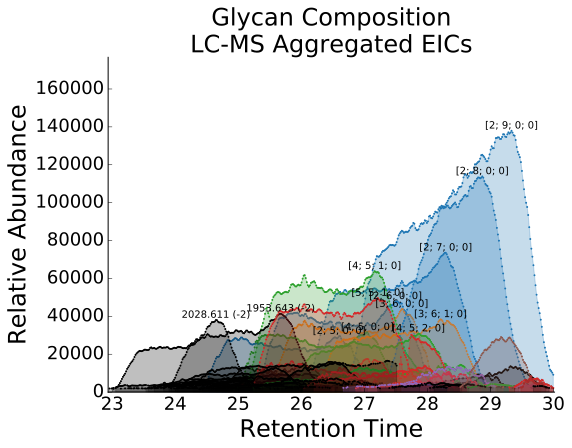
\includegraphics[width=0.45\textwidth,valign=t]{figure/phil_bs_chromatograms.pdf}
        \includegraphics[width=0.45\textwidth,valign=t]{figure/phil_bs_abundances.pdf}
    \end{figure}

    \begin{figure}[!htb]
        \caption{Performance Comparison with and without Network Smoothing for \philbs
                 \label{fig:philbs_perf}}
        \centering
        \includegraphics[width=0.42\textwidth,valign=t]{figure/phil_bs_native_roc.pdf}
        \includegraphics[width=0.45\textwidth,valign=t]{figure/phil_bs_native_prec_rec.pdf}
    \end{figure}

    The comparison of assignment performance with differing degrees of smoothing is
    shown in Figure~\ref{fig:philbs_perf}. The ROC AUC for the unregularized condition is
    0.838, for the partially regularized condition is 0.987, and for the fully regularized
    condition is 0.921. This demonstrates a higher true positive rate at the same false positive
    rate for both regularization conditions compared to the unregularized condition. In
    this condition, the Precision-Recall curve does not show a substantial difference in
    performance between conditions.

\subsection{Chromatogram Assignment Performance for \rpserum}
    The fitted parameters for the network constructed for \rpserum are shown in
    Table~\ref{tab:rpserum_parameters}. The assigned chromatograms are shown in
    Figure~\ref{fig:rpserum_assignments}.

    \begin{figure}[!htb]
        \centering
        \caption{Chromatogram Assignments for \rpserum\label{fig:rpserum_assignments}}
        \begin{minipage}{0.45\linewidth}
            \centering
            \vspace{0pt}
            \includegraphics[width=\linewidth]{figure/rp_serum_chromatograms.pdf}
            \subcaption{Features Assigned After Grid Regularization of \rpserum\label{fig:rpserum_assignment:a}.
            Layout not finalized}
        \end{minipage}
        \begin{minipage}{0.45\linewidth}
            \centering
            \begin{subfigure}[t]{\linewidth}  
                \includegraphics[width=0.75\linewidth, valign=t]{figure/fucosylated_tetra_antennary_structures.pdf}
                \subcaption{
                    Low scoring features which may be discarded based on individual evidence alone
                    may be more reasonable to accept given evidence from related composition, such
                    as our network smoothing method.\label{fig:rpserum_assignment:b}
                }
            \end{subfigure}

            \begin{subfigure}[t]{\linewidth}
                \includegraphics[width=0.75\linewidth, valign=t]{figure/ammonium_adduct_ambiguity.pdf}
                \subcaption{
                    This sample contains heavy ammonium adduction which introduces ambiguity
                    in intact mass based assignments.\label{fig:rpserum_assignment:c}
                }
            \end{subfigure}
        \end{minipage}
    \end{figure}

    \begin{figure}[htb]
        \caption{Performance Comparison with and without Network Smoothing for \rpserum
                 \label{fig:rpserum_perf}}
        \centering
        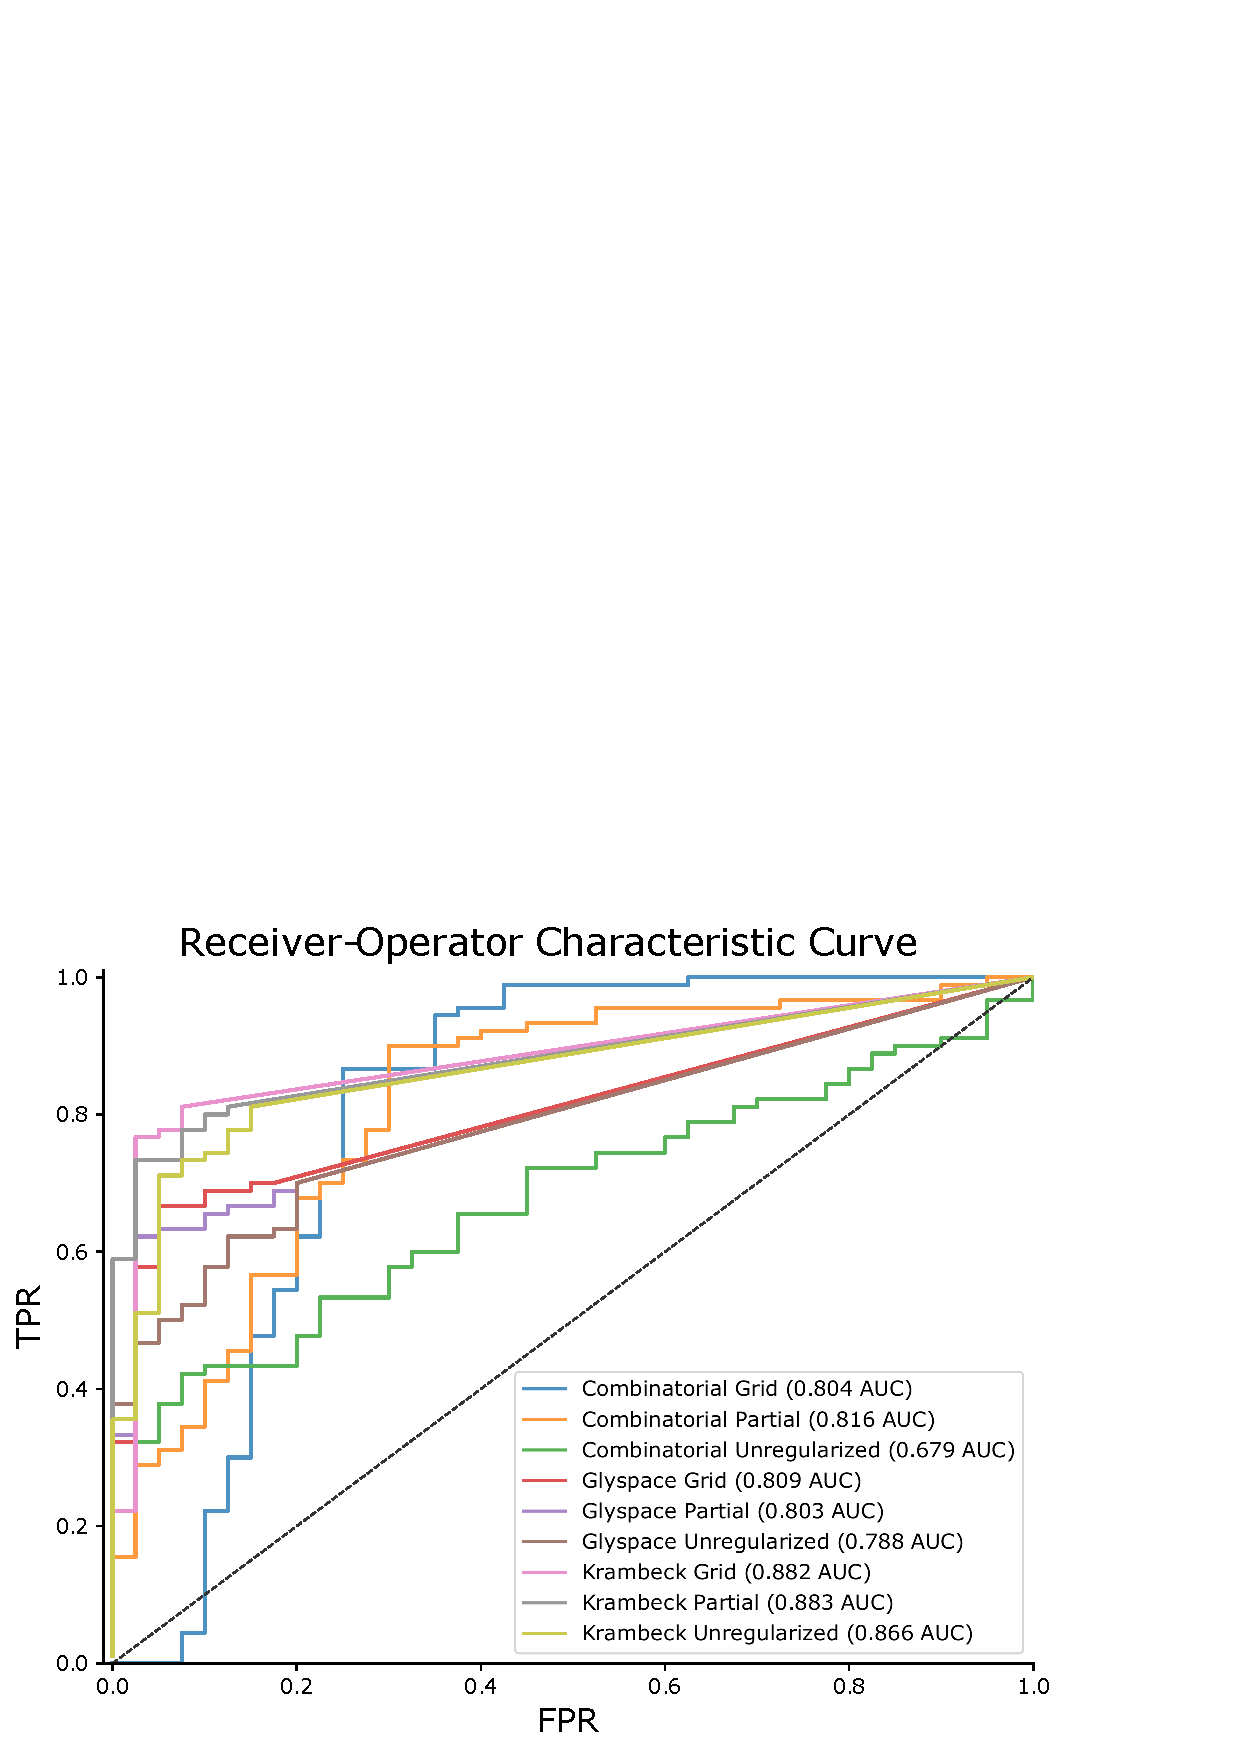
\includegraphics[width=0.42\textwidth,valign=t]{figure/serum_roc.pdf}
        \includegraphics[width=0.45\textwidth,valign=t]{figure/serum_prec_rec.pdf}
    \end{figure}

    The comparison of assignment performance with differing degrees of smoothing is
    shown in Figure~\ref{fig:rpserum_perf}. The ROC AUC for the unregularized condition
    is 0.719, for the partially regularized condition is 0.835, and for the fully
    regularized condition is 0.791. The Precision-Recall AUC for the unregularized condition
    is 0.834, for the partially regularized condition is 0.896, and for the fully regularized
    condition is 0.852. This demonstrates that the partially regularized condition has superior
    performance to the unregularized and fully regularized conditions. This is complicated by
    the redundancies caused by ammonium adduction, but without high quality \msn this cannot
    be resolved.


% \section{Discussion}

\subsection{Glycan Assignment Performance}

    \subsubsection{IgG}
        In \igg and \agp the known common glycoforms were assigned without ambiguity,
    both with and without formate adducts, confirmed manually. In these cases,
    network smoothing is not necessary. The estimates of $\mathbf{\tau}$ in \igg
    are low because the number of glycan compositions observed is low and the overlap
    in $\mathbf{A}$ is large.

    \subsubsection{Alpha-1 Acid Glycoprotein}
        In \agp, there are many more compositions to assign, which in turn leads to
    larger $\mathbf{\tau}$ estimates, with good support for all observations with the
    exception of \texttt{\{Hex:5; HexNAc:4; Neu5Ac:1\}} which depends upon the
    asialo-bi-antennary neighborhoods, and is also the only observed member of this
    neighborhoods. The related sample \dpagp, shows similar distributions for tri-,
    tetra, and penta-antennary forms with low abundance of the bi-antennary forms. The
    low abundance mono-sialylated tetra-antennary case is 


    \subsubsection{Influenza Strains}
        In \phil, the unregularized case contains some ambiguous matches where the biological
    context implies they should not be possible, \texttt{\{Hex:7; HexNAc:6; Neu5Ac:4\}}, or
    where the biological context and neighboring observations support the presence of a glycan
    composition but the evidence does not satisfy the scoring function, \texttt{\{Hex:10; HexNAc:2\}},
    \texttt{\{Hex:6; HexNAc:5\}}, and \texttt{\{Fuc:1; Hex:7; HexNAc:6\}}. By applying the smoothing
    procedure with the parameters automatically estimated with grid search (Table \ref{tbl:phil_82_score_table}),
    \texttt{\{Hex:7; HexNAc:6; Neu5Ac:4\}} was eliminated, while \texttt{\{Hex:10; HexNAc:2\}} and
    \texttt{\{Hex:6; HexNAc:5\}} were boosted into a higher confidence score range. The change
    to \texttt{\{Fuc:1; Hex:7; HexNAc:6\}} was insufficient to reach a high confidence score range,
    and the score for \texttt{\{Fuc:1; Hex:8; HexNAc:7\}} was dropped from a plausible score range
    to a low confidence range. Both these larger asialo-\nglycans have been previously assigned
    in \cite{Khatri2016a},  but the automated procedure drops these compositions while estimating
    ${\hat \gamma}$ leading to empty neighborhoodss when estimating $\mathbf{\tau}$. A user-generated
    $\mathbf{\tau}$ would contain a value greater than 5 in those neighborhoods.
    \todo[inline]{This would be another table entry in \verb|tbl:phil82_score_table|, already computed but
    uncertain how to integrate into the flow yet}

        We are justified in \texttt{\{Hex:7; HexNAc:6; Neu5Ac:4\}}'s removal based on its lack of supporting
    intermediary glycoforms and relatives above the selected $\hat{\gamma}$. If its own score exceeded $\hat{\gamma}$,
    it would itself result in a non-zero value for its related neighborhoods, providing itself with a
    non-zero minimum value and adjusting its rate of decay with $\lambda$. This is not to say that the
    LC-MS evidence that was observed is not real signal, merely that the assignment of that signal the
    glycan composition \texttt{\{Hex:7; HexNAc:6; Neu5Ac:4\}} is unlikely given the context.

        The related \dpphil sample we see a similar pattern of glycoforms though with a wider range of
    fucosylation. In this case, we also have chemical noise from permethylation and a low degree of
    ammonium adduction, which can lead to more spurious matches. We match several multiply
    sialylated glycan compositions in this sample which do not satisfy any of the neighborhood conditions
    in Table \ref{tbl:neighborhood_definitions}, which results in their score decaying rapidly as $\lambda\rightarrow1$.
    If these compositions were viable under the user's glycome model, then a different set of neighborhood
    rules would need to be specified which covered this group. In this case, several of them are ambiguous
    assignments of the same signal due to the mass shift imposed by ammonium ($17.026$ Da, \texttt{H3 N1}) compared to a proton
    adduct, is nearly the same as the difference between a permethylated \monosaccharide{Neu5Ac} and permethylated
    \monosaccharide{FucHex} ($17.015$ Da, \texttt{H3 C1 O1 N-1}). In other cases, monosialylated compositions
    are either not eliminated or receive a larger score after smoothing because they are connected to the
    asialo neighborhoods, which are strongly supported in this glycome. We manually confirmed that the
    signal assigned to \texttt{\{{Fuc:1; Hex:5; HexNAc:4; Neu5NAc:1}\}} is not a deconvolution artefact,
    but the signal for \texttt{\{{Fuc:2; Hex:5; HexNAc:4; Neu5NAc:1}\}} is partially overlapped and 
    difficult to manually separate. While this connection between monosialo and asialo forms may make sense
    in some cases, the link may not be appropriate for the biological context of this sample where
    a viral protein Neuraminadase removes \monosaccharide{Neu5Ac}, and the user could redefine the
    neighborhoods to omit that overlap. Similar commentary can be made for \philbs, which while not
    permethylated and ammoniated, shows the presence of sialylated compositions due to variable adduction.

    \subsection{Utility of Network Smoothing}



\bibliographystyle{natbib}
\bibliography{bibliography}

\end{document}